\documentclass{scrartcl}

\usepackage{scrhack}

\usepackage[aux]{rerunfilecheck}

\usepackage{polyglossia}
\setmainlanguage{german}

\usepackage{fontspec}

\usepackage{float}
\floatplacement{figure}{htbp}
\usepackage[
  section,
  below,
]{placeins}

\usepackage[
  labelfont=bf,
  font=small
  justification=raggedright
  width=0.9\textwidth,
]{caption}
\usepackage{subcaption}
\usepackage{blindtext}

\usepackage{graphicx}
\usepackage{grffile}

\usepackage[unicode]{hyperref}
\usepackage{bookmark}
\pagenumbering{gobble}

\begin {document}
\textbf{\Large{3. Versuchsaufbau und Daten der Probestäbe}}
\newline
\newline
\begin{figure}
  \centering
  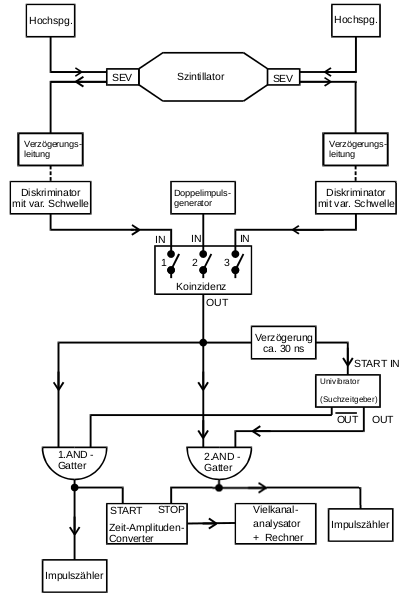
\includegraphics[width=\textwidth]{aufbau.png}
  \caption{Versuchsaufbau [1]}
  \label{fig:bild1}
\end{figure}

 \newline


 \newline




\begin{figure}
  \centering
  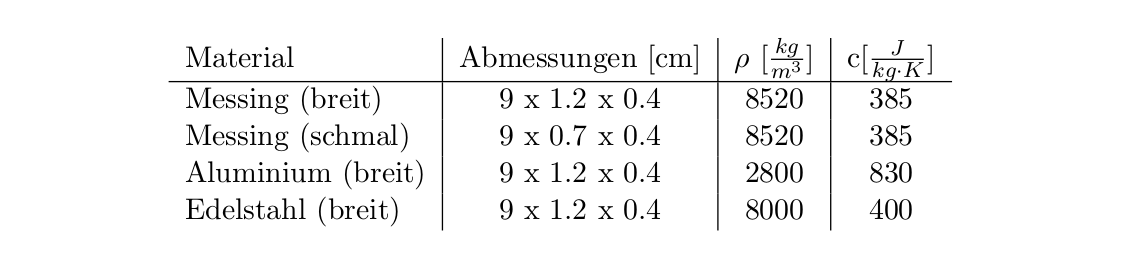
\includegraphics[width=\textwidth]{abmessungen.png}
  \caption{Abmessung der Probestäbe nach [1]}
  \label{fig:bild1}
\end{figure}
\end {document}
